\documentclass[conference]{IEEEtran}
\IEEEoverridecommandlockouts
% The preceding line is only needed to identify funding in the first footnote. If that is unneeded, please comment it out.
\usepackage{cite}
\usepackage{bm}
\usepackage{amsmath,amssymb,amsfonts}
\usepackage{algorithmic}
\usepackage{graphicx}
\usepackage{textcomp}
\usepackage{xcolor}
\def\BibTeX{{\rm B\kern-.05em{\sc i\kern-.025em b}\kern-.08em
    T\kern-.1667em\lower.7ex\hbox{E}\kern-.125emX}}
\begin{document}

\title{Dynamic I/O Model Recommendation System With Machine Learning\\
{\footnotesize \textsuperscript{*}Note: Sub-titles are not captured in Xplore and
should not be used}
\thanks{Identify applicable funding agency here. If none, delete this.}
}

\author{\IEEEauthorblockN{1\textsuperscript{st} Given Name Surname}
    \IEEEauthorblockA{\textit{dept. name of organization (of Aff.)} \\
        \textit{name of organization (of Aff.)}\\
        City, Country \\
        email address or ORCID}
    \and
    \IEEEauthorblockN{2\textsuperscript{nd} Given Name Surname}
    \IEEEauthorblockA{\textit{dept. name of organization (of Aff.)} \\
        \textit{name of organization (of Aff.)}\\
        City, Country \\
        email address or ORCID}
}

\maketitle

\begin{abstract}
    In a typical database and file system, using asynchronous I/O is generally a good way to optimize processing efficiency.
    However, asynchronous I/O may not a more efficient way in all situations.
    In this work, we use Machine Learning(ML) techniques to learn I/O model's performance, and set up a client/server system to recommend the more efficient I/O model under different system loads.
    The experimental result shows that our system has a 15\% performance improvement compared to using asynchronous I/O alone.

\end{abstract}

\renewcommand\IEEEkeywordsname{Keywords}
\begin{IEEEkeywords}
    asynchronous I/O, synchronous I/O, Machine Learning, performance prediction
\end{IEEEkeywords}

\section{Introduction}

% \begin{itemize}
%     \item Data center is popular and I/O is one of the bottlenecks
%     \item asynchronous and synchronous I/O
%     \item Machine Learning
%     \item structure of my system
% \end{itemize}
    
With revolution of “Big Data”, data has grown exponentially in data centers. 
Therefore, data center has to process hundreds of millions of pictures and hundreds of billions of messages each day.
How to improve processing efficiency is a hot issue of a data center. 
Due to the huge speed gap between CPU and I/O device, I/O is one of the bottlenecks of the issue.
Using asynchronous I/O is a common way to boost I/O speed, however, it isn't in all situations of system loads. 

Synchronous and asynchronous I/O are two types of I/O synchronizations as  \emph{\textbf{\large{figure 1}}} shows. 
In a synchronous I/O job, it starts a thread for I/O operation, and it would hang immediately until the operation is finished.
While in a asynchronous I/O job, it would start a thread to send a I/O request to Kernel by calling a function, if the request is accepted successfully, it continues to process other jobs. 
The kernel signals the calling thread when the operation is finished, then the thread interrupts its current job and processes the data from the I/O operation as soon as possible.
Even if it is based on \emph{\textbf{io-uring}},

To help improve system processing efficiency, we purpose to using a recommendation system based on Machine Learning(ML)
This system is running as a daemon like a server and the process requesting the I/O is the client, it collects system I/O data for Machine Learning's training data,
and decide what I/O synchronizations the process uses.

The main challenge of our system is performance, so ...

In summary:
\begin{enumerate}
    \item lightweight
    \item respond 
    \item Self-optimization
\end{enumerate}


\begin{figure}[htbp]
        \centering
        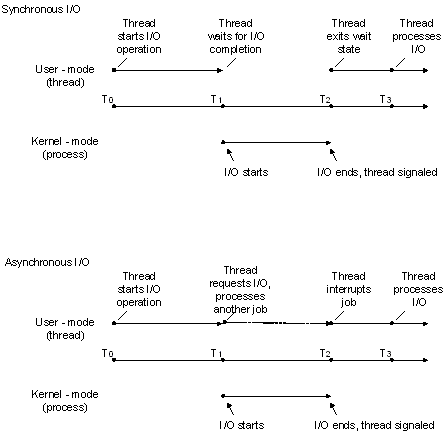
\includegraphics[width=0.45\textwidth]{fig2bedit.png}
        \caption{Asynchronous and Synchronous I/O}
        % \label{fig}
\end{figure}



\section{Design}
\begin{itemize}
    \item evaluate io-uring performance and compare to other ioengins and synchronous
    \item why choosing machine learning and decision-tree
    \item how to connect client and server
\end{itemize}


% \subsection{Maintaining the Integrity of the Specifications}


\section{Implementation}
\begin{itemize}
    \item collect data
    \item train data
    \item build the system
    \item test the system
\end{itemize}

% \subsection{Abbreviations and Acronyms}\label{AA}

% \subsection{Units}
% \begin{itemize}
%     \item Use 
%     \item Avoid.
%     \item Do 
%     \item Use 
% \end{itemize}

% \subsection{Equations}
% \begin{equation}
%     a+b=\gamma\label{eq}
% \end{equation}

% \subsection{Figures and Tables}
% \paragraph{Positioning Figures and Tables} Place figures and tables at the top and

% \begin{table}[htbp]
%     \caption{Table Type Styles}
%     \begin{center}
%         \begin{tabular}{|c|c|c|c|}
%             \hline
%             \textbf{Table} & \multicolumn{3}{|c|}{\textbf{Table Column Head}}                                                         \\
%             \cline{2-4}
%             \textbf{Head}  & \textbf{\textit{Table column subhead}}           & \textbf{\textit{Subhead}} & \textbf{\textit{Subhead}} \\
%             \hline
%             copy           & More table copy$^{\mathrm{a}}$                   &                           &                           \\
%             \hline
%             \multicolumn{4}{l}{$^{\mathrm{a}}$Sample of a Table footnote.}
%         \end{tabular}
%         \label{tab1}
%     \end{center}
% \end{table}

% \begin{figure}[htbp]
%     \centerline{
\includegraphics{fig1.png}}
%     \caption{Example of a figure caption.}
%     \label{fig}
% \end{figure}


\section{Evaluation}
\begin{itemize}
    \item io-uring performance
    \item compare single I/O work performance between used and none-used our system 
    \item compare multi I/O works performance between used and none-used our system 
\end{itemize}

\section{Related Work}
\begin{itemize}
    \item hot issue in I/O
\end{itemize}

\section{Conclusion}
    improvement of our system and future usage scenario

\section*{Acknowledgment}


% \section*{References}


\begin{thebibliography}{00}
    \bibitem{b1} G. Eason, B. Noble, and I. N. Sneddon, ``On certain integrals of Lipschitz-Hankel type involving products of Bessel functions,'' Phil. Trans. Roy. Soc. London, vol. A247, pp. 529--551, April 1955.
\end{thebibliography}
\vspace{12pt}
\color{red}
IEEE conference templates contain guidance text for composing and formatting conference papers. Please ensure that all template text is removed from your conference paper prior to submission to the conference. Failure to remove the template text from your paper may result in your paper not being published.

\end{document}
